\glsresetall

\section{Changes in Microbial Ecology after Fecal Microbiota Transplantation for recurrent \textit{C. difficile} Infection Affected by Underlying Inflammatory Bowel Disease}

\subsubsection{Background}
Gut microbiota play a key role in maintaining homeostasis in the human gut. Alterations in the gut microbial ecosystem predispose to \gls{cdi}, and gut inflammatory disorders such as \gls{ibd}. \Gls{fmt} from a healthy donor can restore gut microbial diversity and pathogen colonization resistance; consequently it is now being investigated for its ability to improve inflammatory gut conditions such as \gls{ibd}.  In this study, we investigated changes in gut microbiota following \gls{fmt} in 38 patients with \gls{cdi} with or without underlying \gls{ibd}. 

\subsubsection{Results}
There was a significant change in gut microbial composition towards the donor microbiota, and an overall increase in microbial diversity consistent with previous studies after \gls{fmt}. \gls{fmt} was successful in treating \gls{cdi} using a diverse set of donors, and varying degrees of donor stool engraftment suggesting that donor type and degree of engraftment are not drivers of a successful \gls{fmt} treatment of \gls{cdi}. However, patients with underlying \gls{ibd} experienced an increased number of \gls{cdi} relapses (during a 24-month follow-up), and a decreased growth of new taxa, as compared to the subjects without \gls{ibd}, note that the test used presents some limitations in sample size and statistical assumptions (see methods). Moreover, the need for \gls{ibd} therapy did not change following \gls{fmt}. These results underscore the importance of the existing gut microbial landscape as a decisive factor to successfully treat \gls{cdi}, and potentially for improvement of the underlying pathophysiology in \gls{ibd}. 

\subsubsection{Conclusions}
\Gls{fmt} leads to a significant change in microbial diversity in patients with recurrent \gls{cdi} and complete resolution of symptoms. Stool donor type (related or unrelated) and degree of engraftment are not key for successful treatment of \gls{cdi} by \gls{fmt}. However, \gls{cdi} patients with \gls{ibd} have higher proportion of the original community after \gls{fmt} and lack of improvement of their \gls{ibd} symptoms and increased episodes of \gls{cdi} on long-term follow-up.

\subsubsection{Keywords}
Fecal microbiota transplantation, microbiome, Clostridium difficile infection, inflammatory bowel disease

\subsection{Background}

Gut microbiota play a key role in maintaining homeostatic host functions and deleterious shifts in the gut microbial ecosystem, often referred to as dysbiosis, are associated with \gls{cdi}, \gls{ibd} and other systemic inflammatory conditions \cite{RN1477}. A diverse gut microbial community confers colonization resistance against pathogens such as \textit{C. difficile}, and disruption of a diverse community structure from antibiotics, comorbidities, altered gastrointestinal transit or other risk factors can lead to pathogen colonization and infection \cite{RN1480}.

With increasing incidence of community and hospital acquired \gls{cdi}, high rates of recurrent \gls{cdi} (estimated 20-30\% after a first and 50-60\% after a third infection), high mortality (~29,000 deaths annually) in the United States, and an urgent need for newer non-antibiotic therapies has led to the emergence of microbiome based therapies \cite{RN1478}. \Gls{fmt} in \gls{cdi} patients restores phylogenetic diversity to levels more typical of a healthy person, with response rates $>$85\% by enema, oral capsule or endoscopic delivery modes \cite{RN1484, RN1479, RN1481}. A recent study suggests significantly lower response of \gls{cdi} to \gls{fmt} in patients with underlying \gls{ibd} \cite{RN1497}. We have also previously described a higher rate of recurrence of \gls{cdi} following \gls{fmt} in patients with \gls{cdi} and underlying \gls{ibd} \cite{RN1498}. It remains unclear if changes in gut microbial ecology play a role in long-term success of \gls{fmt} in these patients.

\Gls{fmt} has not shown consistent success in treating other diseases associated with microbial dysbiosis such as \gls{ibd}. Three clinical trials to treat \gls{uc} with \gls{fmt} have shown conflicting results and one highlighted the potential role of specific gut microbial members in donor stool in determining success after \gls{fmt} in \glspl{uc} \cite{RN3982, RN1019, RN1483}.  The underlying host or donor factors that may be important for success of \gls{fmt} in treatment of \gls{ibd} remain unclear.

In this study, we assessed the effect of donor type (standard donor versus related donor) and changes in gut microbial ecology on response to \gls{fmt} in \gls{rcdi} with and without underlying \gls{ibd} as well as clinical response to \gls{fmt}. 

\subsection{Methods}
\subsubsection{Patient selection}
Patients undergoing \gls{fmt} for \gls{rcdi} were prospectively recruited in this study. Informed consent was obtained to collect clinical data and stool samples. Data collected included demographics, clinical history, \gls{cdi} treatment history, comorbid conditions and response to \gls{fmt}. A donor fecal sample was collected prior to \gls{fmt}. Stool samples from the recipients were collected before \gls{fmt}, and at day 7 and day 28 and were stored at -80\textdegree C. The donors were either related (genetically related family members) or unrelated (screened hospital employee volunteer donors or unrelated family members) and a fresh sample was obtained on the day of \gls{fmt}. All donors underwent extensive screening in accordance with standard practice and guidelines from the Food and Drug Administration \cite{RN1446}. Donor selection criteria and experience from our group have been previously published \cite{RN1523}. The donor stool sample is weighed and divided into 50 grams aliquots. Each aliquot of 50 grams is diluted in normal saline in a 1:5 ratio (50 grams of stool diluted with 250 ml of normal saline) and is placed in the blender bag (a 2 bag system with a semipermeable membrane in the inner bag and the outside bag is plastic). The stool is placed in the inner bag and normal saline is added. The bag is placed in a sealed compartment in the stomacher 400 (Seward) and blended for 60 seconds at 230 rotations per minute. The filtrate is then placed into 50 ml conical tubes using 50 ml pipettes and placed on an ice pack prior to the procedure.  \Gls{rcdi} was defined as another episode of \gls{cdi} within 56 days after symptom resolution with recurrence of symptoms and a positive stool polymerase chain reaction test. For this study, future \textit{C. difficile} episodes after \gls{fmt} up to 2 years were captured. These were categorized as up to 56 days, 56 days to 1 year and beyond 1 year. 

\subsubsection{Sequencing and analytic methods}
After fecal DNA isolation (MoBio, Carlsbad, CA fecal DNA kit), amplicons spanning the variable region 4 of bacterial 16S rRNA were generated and sequenced using Illumina MiSeq platform at the Mayo Clinic Medical Genome Facility, Rochester, MN. The 16S rRNA sequencing data from the Illumina runs were quality controlled, trimmed, demultiplexed and assigned to \glspl{otu} following the closed reference at 97\% similarity (using SortMeRNA as a clustering algorithm \cite{RN3810} protocol against the Greengenes \cite{RN1516fmt} database 13\textunderscore 8 release, as implemented in \gls{qiime} 1.9.0 software \cite{RN41200}, default parameters were used for all these steps unless otherwise noted. After quality control, 10,583,052 sequences were obtained, for a mean of 76,688 sequences per sample (min: 33,559, max: 154,200).

 Alpha diversity values were calculated using Faith's phylogenetic diversity \cite{RN4007}. To assess differential abundance between the groups, we used ANCOM \cite{RN1513}, as implemented in scikit-bio 0.5.1\footnote{\url{http://scikit-bio.org/docs/0.5.1/}}. This is tested by looking at the individual \glspl{otu} across the patient types (with and without underlying \gls{ibd}); \glspl{otu} of the same genus are grouped for displaying purposes. We note that ANCOM makes the statistical assumption that fewer than 25\% of taxa change, not met in all these comparisons (before \gls{fmt} and post \gls{fmt} communities are expected to be very different \cite{RN1471}).
 
The donor-plane is created using all the donor samples, and serves as a proxy for where their microbiomes are in the ordination space, and how as time goes by this proximity changes. This procedure was originally presented by Halfvarson et al. \cite{RN1515}.

Beta diversity matrices were created using unweighted UniFrac \cite{RN83}, and plotted using Emperor \cite{RN1501} (all other plotting was done using the Seaborn visualization package).

Processed tables and sample information can be found in Qiita\footnote{\url{https://qiita.ucsd.edu}} under study id 10057, alternatively the data can be found under accession number ERP021216 at the European Bioinformatics Institute.

\subsubsection{SourceTracker Analysis}
To assess the proportion of pre-transplant communities that were retained in the patients' microbiota, we used SourceTracker \cite{RN3995}. The pre-transplant samples and the donor samples were described as \textit{sources}; all the other samples were used as \textit{sinks}. For all samples at day seven and twenty-eight, SourceTracker estimated the proportion of communities that were attributed one of three environments, (1) the donor, (2) the patient pre-transplant, and (3) and unknown community. Using these proportions, we grouped the samples according to their \gls{ibd} status and compared their distributions using the Mann-Whitney test (as implemented in SciPy 0.15.1\cite{RN1516fmt}).

\subsubsection{Clinical Statistics}
Statistical analyses for clinical data were performed with JMP version 11.0 (SAS institute, NC).  Data analysis included descriptive statistics, t-tests for normally distributed variables, non-parametric tests for skewed variables, chi-square tests and ANOVA tests as applicable. A p-value less than 0.05 was considered statistically significant


\subsection{Results}

\subsubsection{FMT leads to resolution of CDI}
In order to assess gut microbiota changes following \gls{fmt}, 38 patients with recurrent \gls{cdi} were enrolled in the study and a fecal sample was obtained prior to transplant, as well as 7 and 28 days post-transplant. Sample handling, donor and recipient sample collection, sample processing and data analyses are detailed in supplementary methods. \gls{fmt} was accomplished by colonoscopy using fresh donor stools from related (n=12) or unrelated (n=26) donors. None of the \gls{ibd} patients received stool from a related donor. The demographic, disease and treatment characteristics are outlined in Table~\ref{fmt-tab1}. Detailed characteristics of \gls{ibd} patients are shown in supplementary table 1. Twelve patients (31.6\%) had \gls{ibd} (6 with \glspl{uc} and 6 with Crohn's disease), with median age 27.6 years (range, 23.3-74.9), and median \gls{ibd} duration 5 years (range, 2-33). 58.3\% percent of patients were on 5-ASA (amino salicylic acid) agents, 50\% on biologics and 33.3\% on immunomodulators and 58.3\% on steroids.  Among patients with \gls{ibd}, at the time of colonoscopy, 2 had normal colonoscopy, 1 had pseudopolyps, 5 had severe pancolitis, 1 had moderate colitis, 1 had mild colitis, 1 had mild procto-sigmoiditis and 1 had moderate ileo-colitis (Supplementary Table 1).

\begin{sidewaystable}[hbtp]
    \centering
    \renewcommand{\arraystretch}{0.65}% Tighter
    \caption{Clinical Characteristics}
    \begin{tabular}{P{9cm}P{2cm}P{2cm}P{2cm}P{2cm}}
     \toprule
      & & Overall (n=38) &	IBD (n=12) &	No IBD (n=26) \\
    \midrule
   \multirow{2}{9cm}{Age} & median & 53.1  &	27.6  &	58.3\\
   & (range) & (21.9-82.7) & (23.3-74.9) & (21.9-82.7)\\
    \midrule
    \multicolumn{2}{l}{Sex distribution (\% female)} &	81.6&	66.7&	88.5\\
    \midrule
    \multirow{2}{9cm}{BMI, kg/m2} & median  &	24.8 & 	25.6 & 23.8\\
    &(range) & (14.9-39.9) & (18.5-30.3) &	(14.9-39.9)\\
    \midrule
    \multirow{2}{9cm}{Number prior CDI episodes} & median & 	5 & 4.5 & 5\\
    & (range) & (3-13) & (3-7) & (3-13)\\
    \midrule
    \multirow{2}{9cm}{Number prior metronidazole courses} & median &	1 & 1 & 1\\
    &(range) & (0-8) & (0-2) & (0-8)\\
    \midrule
    \multirow{2}{9cm}{Number prior vancomycin 10-14 day courses} & median  &	2 & 2 & 2\\
    & (range) & (0-4) & (0-4) &	(0-3)\\
    \midrule
    \multirow{2}{9cm}{Number prior vancomycin tapers} & median  &	1&1&1\\
   & (range) & (0-5) &(0-1)&(0-5)\\
    \midrule
    \multirow{2}{9cm}{Number prior fidaxomicin courses} & median &	0 & 0 & 0\\
    &(range) & (0-4) & (0-2) & (0-4)\\
    \midrule
    \multicolumn{2}{l}{Recurrent CDI after FMT (\%)}&	13.2&	25&	8.4\\
    \bottomrule
    \end{tabular}
    \label{fmt-tab1}
\end{sidewaystable}
\renewcommand{\arraystretch}{1}% Restore to default


All patients responded to \gls{fmt} with regards to clinical or microbiologic remission of \gls{cdi} (negative \textit{C. difficile} testing), 92.1\% (n=35) of patient symptoms returned to baseline bowel pattern (as before \gls{cdi}) and resolution of \gls{cdi}, 5.3\% (n=2, both with \gls{ibd}) had worsening diarrhea (\textit{C. difficile} negative), and 2.6\% (n=1) had new onset constipation after \gls{fmt}. Upon long-term follow-up of 24 months; 13.2\% (n=5/38; of these n=1 within 56 days, n=1 from 56 days to 1 year and n=3 beyond 1 year, Supplementary Table 2) had another episode of \gls{cdi} and 10.5\% (n=4/38) required a second \gls{fmt} due to multiply \gls{rcdi}. One patient with \gls{rcdi} was treated with vancomycin. The risk of another episode of \gls{cdi} after \gls{fmt} in \gls{ibd} patients was 25\% (n=3/12) compared to 7.7\% (n=2/26) in non-\gls{ibd} patients (p=0.16, chi-square test). Seven of the 12 patients with \gls{ibd} were on systemic immunosuppression. None of the patients with \gls{ibd} had improvement in their \gls{ibd} course after \gls{fmt}, and none were able to withhold, de-escalate or stop \gls{ibd} treatment. This is not an unexpected finding as one time \gls{fmt} would not be expected to alter the disease course in \gls{ibd} patients.

\subsubsection{FMT decreases microbial dysbiosis}
\gls{fmt} led to a significant increase in alpha diversity based on Faith's phylogenetic diversity, Shannon's diversity index and observed species, both at day 7 and day 28 (Mann-Whitney p$<$0.05; Supplementary Figure~1, comparing pre- and post-\gls{fmt} in patients with \gls{cdi} with or without underlying \gls{ibd}).  Also, patient's stool closely resembled donor stool, as evidenced by a rapid and sustained change in unweighted and weighted UniFrac-based beta diversity following \gls{fmt} at day 7 and 28 post-transplant (Figure~\ref{fmt-fig1}A; PERMANOVA p$<$0.05) \cite{RN83}. 


\begin{sidewaysfigure}[htbp]
\centering
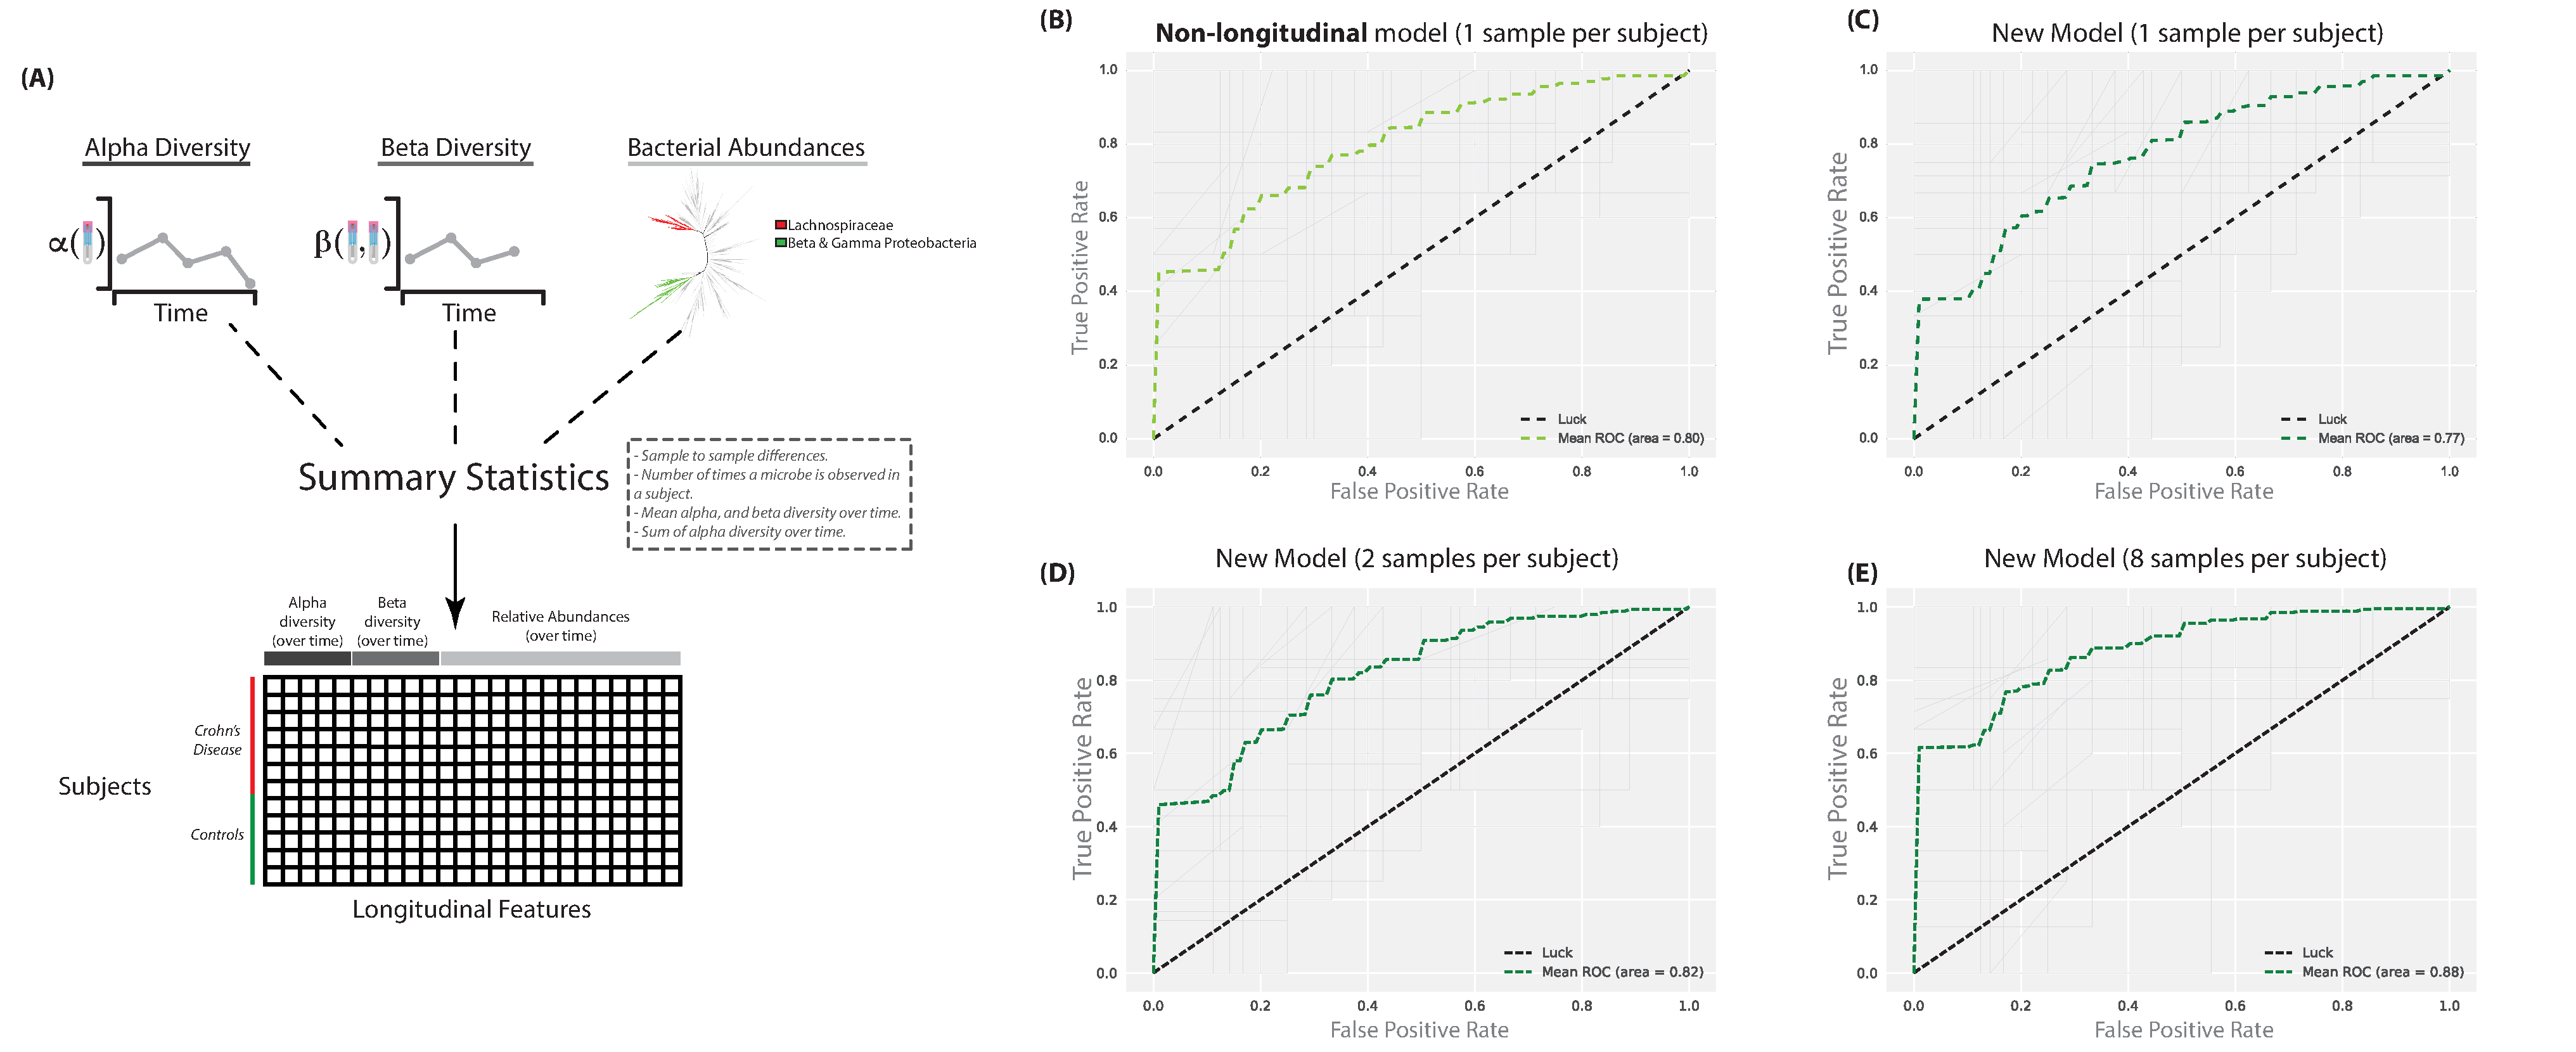
\includegraphics[width=0.8\textheight]{fmt-figures/figure-1}
\caption[Dysbiosis index and beta-diversity summaries pre- and post-fecal microbiota transplantation]{(A) Principal Coordinates Analysis of the unweighted UniFrac distances, showing change in the phylogenetic diversity between patients with CDI, 7 and 28 days after fecal microbiota transplant. (B) Change in dysbiosis index following fecal microbiota transplant in patients with CDI with or without IBD. (C) Spearman correlation to donor stool 7 and 28 days following fecal microbiota transplantation.}
\label{fmt-fig1}
\end{sidewaysfigure}

To characterize the changes in community composition, we use the \gls{md} index as a reference to describe the dominance of individual taxa (Supplementary Table 3). The \glspl{md} index is composed of 18 taxonomic groups, as defined by Gevers et al, with a higher value correlated with greater disease severity in \gls{ibd}, and lower values associated with healthier states \cite{RN154}. As \gls{cdi} is also associated with dysbiosis and inflammation, we wanted to determine the effect of \gls{fmt} on dysbiosis. The \glspl{md} index values were significantly higher in patients with \gls{cdi} compared to donors (Mann-Whittney's U, p $<$ 0.05, Figure~\ref{fmt-fig1}B). However, on day 7 and 28 after the transplantation, the \glspl{md} index values were similar to donors (Mann-Whitney's U p $>$ 0.05, Figure~\ref{fmt-fig1}B) and this change was independent of whether recipients had \gls{ibd} or not. 

In order to determine if the changes seen in our subjects following \gls{fmt} were similar to other published studies we compared our samples with recently published data from Weingarden et al. 2015 (Supplementary Figure 2A) wherein 4 patients with \gls{rcdi} (but not \gls{ibd}) received \gls{fmt} from a single donor \cite{RN1471}. Similar to our findings, there was a rapid and sustained change in beta diversity (Supplementary Figure 2A) following \gls{fmt} and the regression to the donor plane (change in microbial composition to resemble healthy donors) following \gls{fmt} was remarkably similar in the two studies (Supplementary Figure 2B). In this context, we refer to the donor plane as a proxy to the region in the\gls{pcoa}: a dimensionality reduction method to visualize beta-diversity distance matrices) space where the donors are located; we do this by fitting a three-dimensional plane (using the least squares method) to the samples from the donors. As the communities change post-\gls{fmt}, the distance to this plane is reduced.

\subsubsection{Clinical response of CDI to FMT is independent of engraftment or donor type but underlying IBD influences changes in gut microbial ecology after FMT}

In order to determine if the response of \gls{cdi} to \gls{fmt} was dependent on donor stool engraftment, we determined Spearman's correlation coefficient between fecal microbial communities prior to and 7 and 28 days post-transplant. The fecal microbial communities from patients with \gls{cdi} were distinct from donor communities prior to transplant (Spearman's r$<$0.2 for all subjects, Figure~\ref{fmt-fig1}C). Following transplant the communities showed an increase in correlation to donor stool at day 7 (Spearman's r$>$0.4 for 85\% of the subjects, Figure~\ref{fmt-fig1}C) and a spread for all subjects at day 28 ranging from below 0.2 up to 0.6 (Figure~\ref{fmt-fig1}C). Using SourceTracker \cite{RN3995}, we found that after \gls{fmt}, subjects with \gls{ibd} retained a higher proportion of their original communities (Mann-Whitney p $<$ 0.05 at day 7, and p = 0.06 at day 28; Figure~\ref{fmt-fig2}A and \ref{fmt-fig2}B) and a significantly lower proportion of new communities (Mann-Whitney p $<$ 0.05 at day 7 and 28), as compared to the patients without \gls{ibd}. The expansion of new taxa following \gls{fmt} represents a beneficial ecological change following \gls{fmt} as seen in patients without \gls{ibd}, while those with \gls{ibd} are more prone to revert to the original community structure. Consequently, in patients with \gls{ibd} we observed a smaller group of taxa that change significantly seven days after \gls{fmt}. In both groups, \textit{Bacteroides}, and \textit{Faecalibacterium} showed a significant increase in relative abundance, with \textit{Blautia}, only being increased for patients without \gls{ibd}. Additionally, these patients showed a decrease in relative abundance of \textit{Lactobacillus}, \textit{Veillonella}, \textit{Enterobacter}, \textit{Klebsiella}, \textit{Erwina}, \textit{Proteus}, \textit{Salmonella}, and \textit{Trabulsiella} (Figure~\ref{fmt-fig2}C and~\ref{fmt-fig2}D, ANCOM p $<$ 0.05, corrected for multiple comparisons using Bonferroni-Holm's method \cite{RN1513}).

\begin{figure}[htbp]
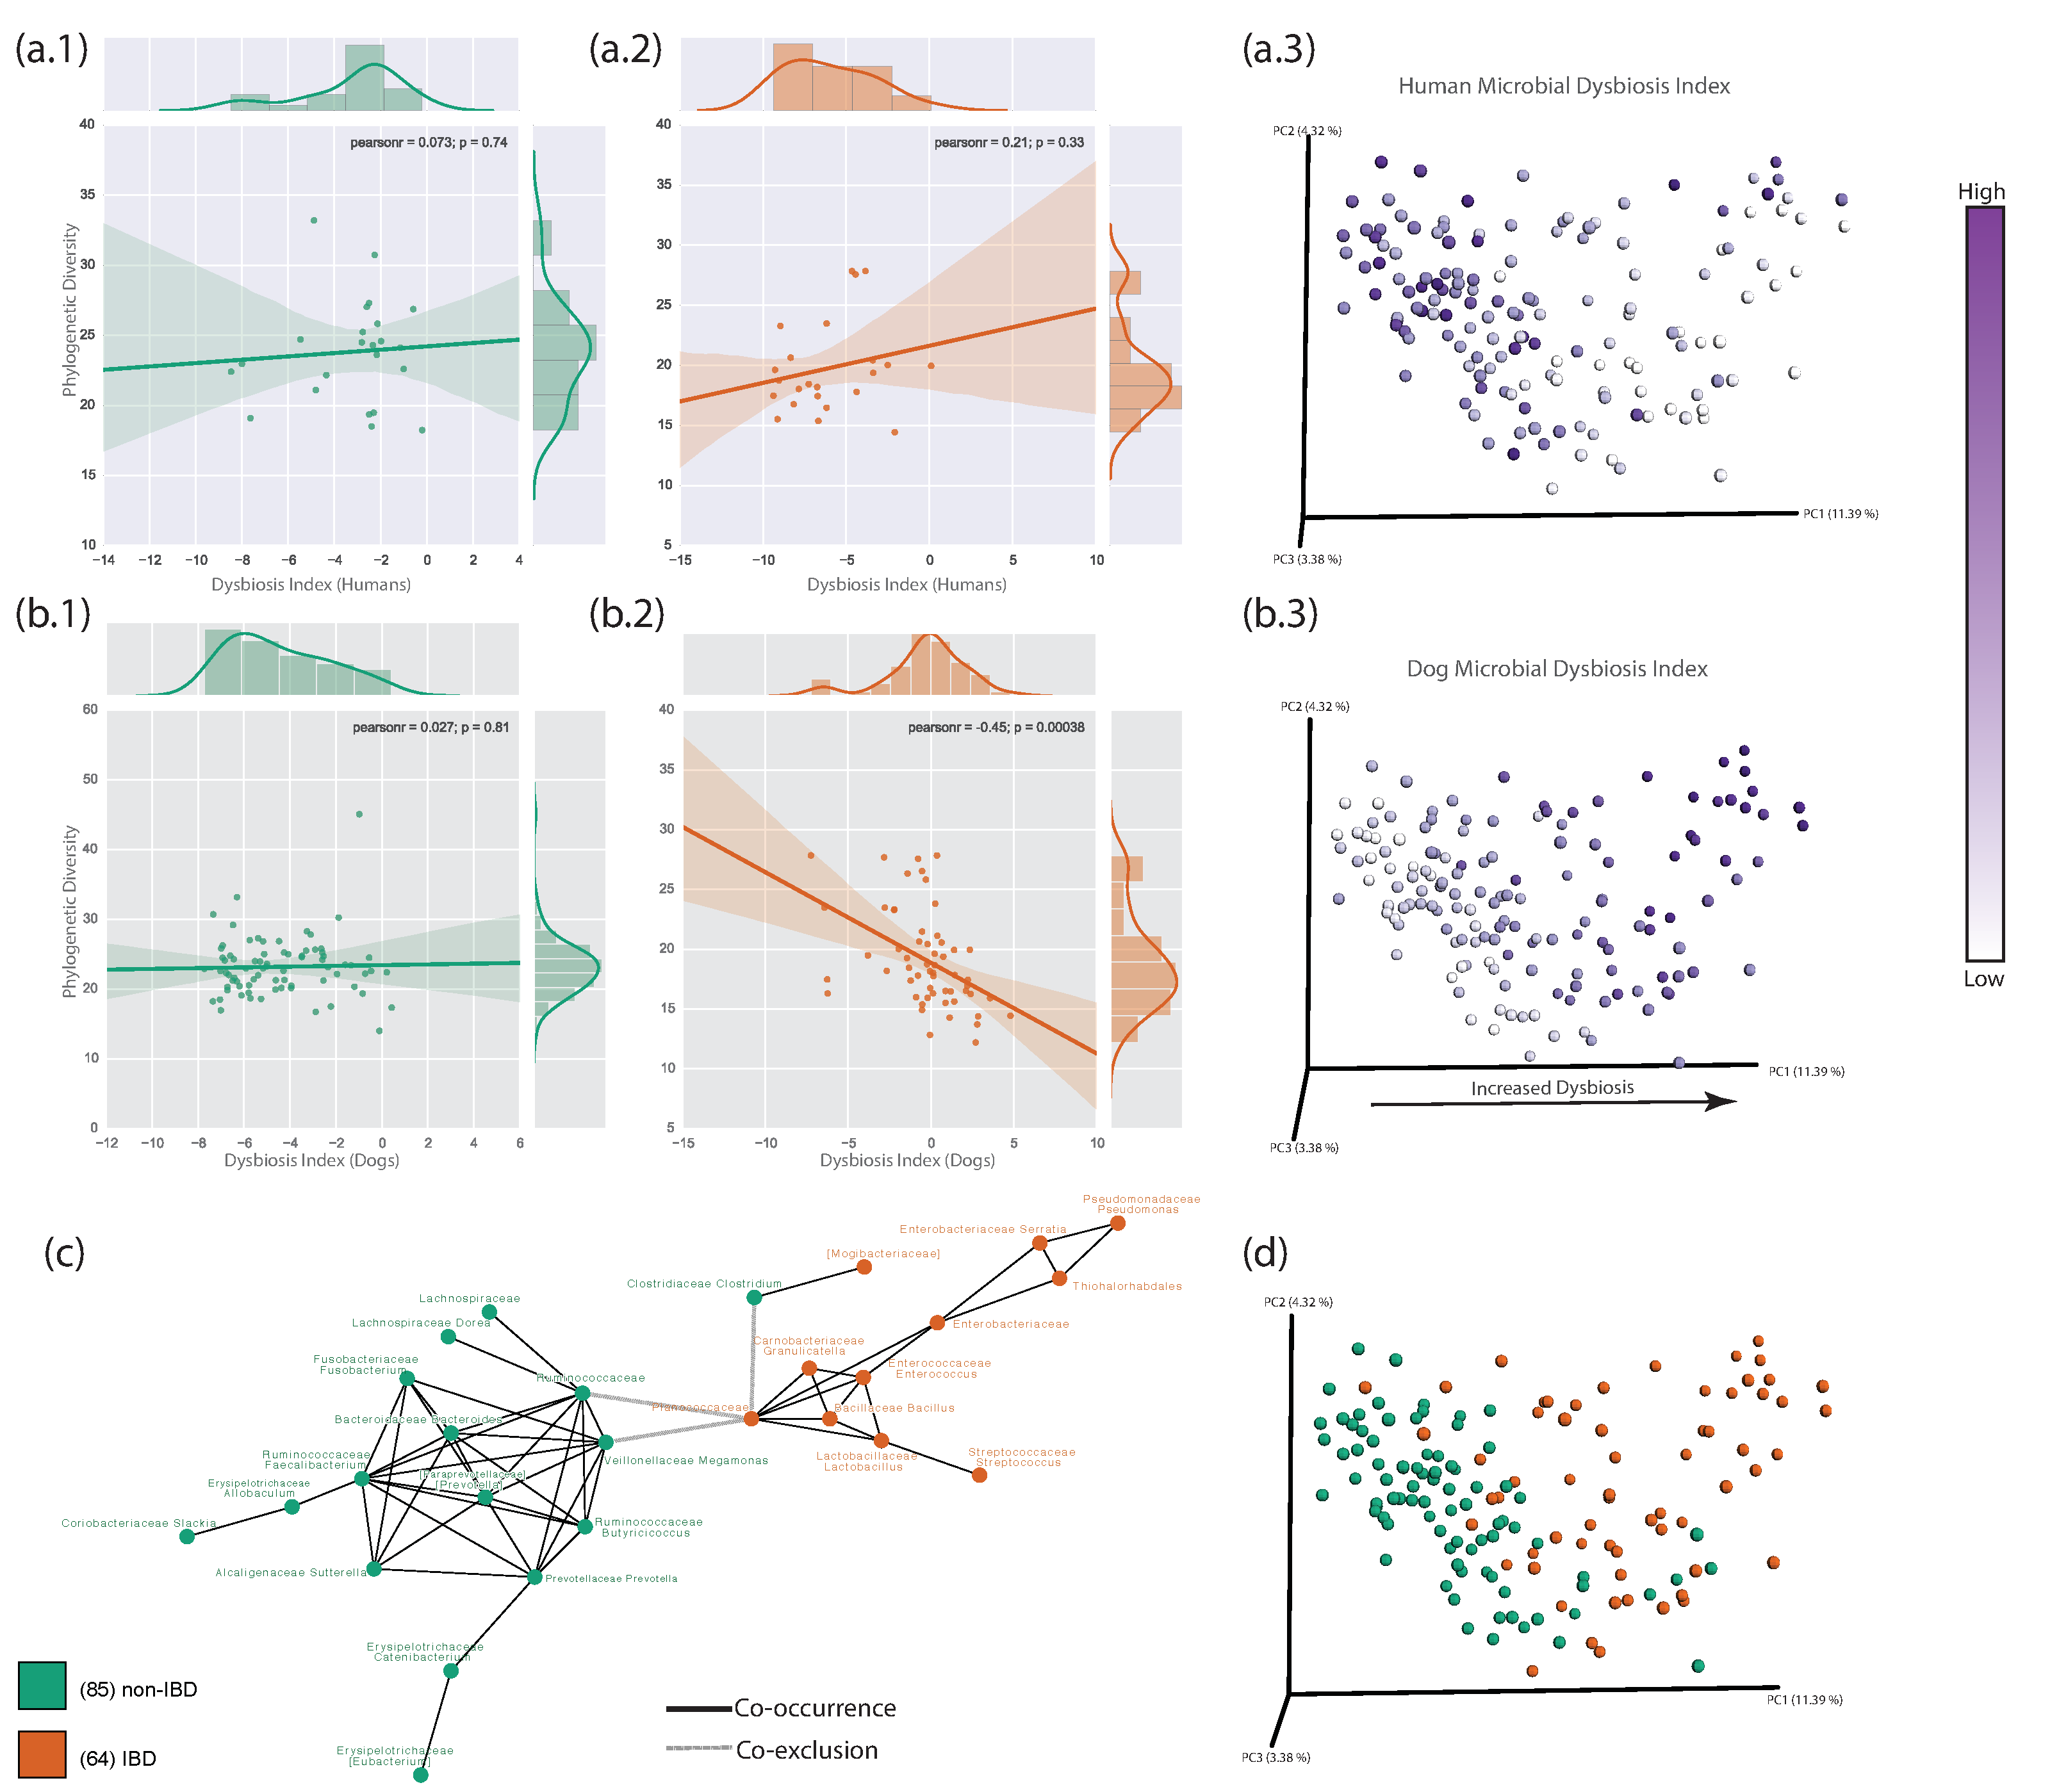
\includegraphics[width=0.95\columnwidth]{fmt-figures/figure-2}
\caption[SourceTracker and differential abundance comparison between IBD and non-IBD affected subjects.]{(A) and (B) Subjects with IBD retain a higher proportion of their original communities (Mann-Whitney p $<$ 0.05 at day 7, and p = 0.06 at day 28 and a significantly lower proportion of new communities (Mann-Whitney p $<$ 0.05 at day 7 and 28), as compared to the patients without IBD using SourceTracker. (C) Bacterial taxa that change significantly in patients with IBD after FMT (ANCOM p $<$ 0.05, corrected for multiple comparisons using Bonferroni-Holm's method). (D) Bacterial taxa that change significantly in patients without IBD after FMT (ANCOM p $<$ 0.05, corrected for multiple comparisons using Bonferroni-Holm's method). (E) Change in phylogenetic diversity based alpha diversity 7 and 28 days following fecal microbiota transplant in patients with CDI with and without IBD (Mann-Whitney's U p $<$ 0.001). }
\label{fmt-fig2}
\end{figure}

All patients had either clinical or microbiological remission, confirming that initial response of \gls{cdi} to \gls{fmt} is not dependent on the degree of donor stool engraftment. In this small cohort of patients, those with underlying \gls{ibd} had higher number of late relapses of \gls{cdi}. We found no significant differences in gut microbiota composition following \gls{fmt} from standard donors or related donors (Mann-Whitney p$>$ 0.05 at day 7 and 28), suggesting that engraftment of donor stool was independent of donor type. Furthermore as all patients had ongoing clinical remission with microbiological response (if measured), donor type does not appear to affect \gls{cdi} related clinical response.

\subsubsection{Change in bacterial diversity after FMT is dependent on underlying IBD.}

\gls{ibd} disease course, as measured by the need for specific \gls{ibd} therapies, did not change after \gls{fmt}, and patients with \gls{cdi} and underlying \gls{ibd} retained a higher proportion of the pre-transplant communities and lower proportion of new communities following \gls{fmt}.  Thus, underlying \gls{ibd} appears to affect the change in gut microbial ecology resulting in a less significant increase in overall diversity. In subjects without \gls{ibd}, Faith's phylogenetic diversity (which measures the total branch length of a phylogenetic tree that a given sample covers \cite{RN1490}) reached a level comparable to healthy donors (Mann-Whitney's U p < 0.001, Figure 2E). The differences in phylogenetic diversity following \gls{fmt} between subjects with and without \gls{ibd} became evident on day 7 and persisted on day 28 (Mann-Whitney, day -1 p = 0.163, day 7 p = 0.0058, and day 27 p = 0.008, Figure 2E). A linear regression of phylogenetic diversity vs \glspl{md} index (Supplementary Figure 3) shows a significantly lower negative correlation between the increase in phylogenetic diversity and the increase of the \glspl{md} index in patients with \gls{ibd} (Pearson's correlation coefficient, \gls{ibd} R=-0.68, No \gls{ibd} R=-0.83; p $<$ 0.0001; Supplementary Figure 3) suggesting a lack of recovery of phylogenetic diversity in patients with \gls{ibd} as the \glspl{md} index improves.

\subsection{Discussion}
In this study, we found that gut microbiota diversity changes rapidly following \gls{fmt} for treatment of \gls{cdi} and resembles donor microbiota diversity, similar to previous studies. A successful response of \gls{cdi} to \gls{fmt} was seen with a diverse group of donors and at levels of engraftment (as measured by correlation to donor stool) varying from 50-94\% (at day 7) and 34-93\% (at day 28) based on the proportion of communities attributed to the donor following \gls{fmt} per SourceTracker, suggesting these are not critical factors in determining response.  Similarly, a recent study that evaluated pre- and post-\gls{fmt} (for recurrent \gls{cdi}) gut microbiome samples from a subset of patients enrolled in a randomized controlled trial \cite{RN1527}, compared donor \gls{fmt} to autologous \gls{fmt} suggested that complete engraftment of donor bacteria may be not necessary, if functionally critical taxa are present in subjects following initial antibiotic therapy for \gls{cdi} \cite{RN1524}. This study excluded patients with \gls{ibd} but was able to compare autologous to donor \gls{fmt} unlike our study. There was a higher number of \gls{rcdi} following \gls{fmt} in patients with \gls{cdi} and \gls{ibd} but this was not statistically significant, likely given the small sample size. However we have previously reported similar findings in a larger cohort of patients with \gls{cdi} and \gls{ibd} \cite{RN1498}, where gut microbiota changes were not monitored. Interestingly, in this cohort all patients had an initial clinical or microbiological remission of \gls{cdi} following \gls{fmt} and we did not see a difference in initial response reported in a recent study \cite{RN1497}, which is also likely due to the smaller sample size of our study and differences in underlying disease characteristics. 

We also did not see changes in need for \gls{ibd} therapy in the subset of patients with \gls{ibd} underlying \gls{cdi}. While dynamic variations can be seen in patients following \gls{fmt} \cite{RN1471}, patients with underlying \gls{ibd} in our study show a higher proportion of the original pre-transplant microbial community and lower recovery of phylogenetic diversity following \gls{fmt} compared to those without \gls{ibd}. This lack of beneficial change in microbial ecology may be relevant for long term response of \gls{cdi} in patients with \gls{ibd} and the lack of clinical response of \gls{ibd} to \gls{fmt} seen in our and previous studies \cite{RN1497}. Future studies designed to study the effect of compositional and functional changes in gut microbiota on clinical outcomes following \gls{fmt} in patients with \gls{ibd} will be needed to definitively address the potential importance of changes in microbial ecology, donor selection \cite{RN3982}, underlying disease characteristics and multiple-dose \glspl{fmt}, in correcting the underlying pathophysiology of \gls{ibd}. 

\subsection{Conclusions}

There is a significant increase in microbial diversity in patients with recurrent \gls{cdi} after \gls{fmt}. Both, the degree of microbial engraftment or donor type (related or unrelated) are not key for successful treatment of \gls{rcdi} by \gls{fmt}. Compared to \gls{cdi} patients without \gls{ibd}, \gls{cdi} patients with \gls{ibd} have higher proportion of the original microbial communities after \gls{fmt} and increased episodes of future \gls{cdi} on long-term follow-up.
